%%%%%%%%%%%%%%%%%%%%%%%%%%%%%%%%%%%%%%%%%%%%%%%%%%%%%%%%%%%%
%%  This Beamer template was created by Cameron Bracken.
%%  Anyone can freely use or modify it for any purpose
%%  without attribution.
%%
%%  http://cameron.bracken.bz/beamer-template
%%
%%  Template Last Modified: January 9, 2009
%%

\documentclass[xcolor=x11names,compress]{beamer}

%% General document %%%%%%%%%%%%%%%%%%%%%%%%%%%%%%%%%%
\usepackage{graphicx}
\usepackage{tikz}
\usepackage[utf8]{inputenc}
\usepackage[labelformat=empty]{caption}
\usetikzlibrary{decorations.fractals}
%%%%%%%%%%%%%%%%%%%%%%%%%%%%%%%%%%%%%%%%%%%%%%%%%%%%%%


%% Beamer Layout %%%%%%%%%%%%%%%%%%%%%%%%%%%%%%%%%%
\useoutertheme[subsection=false,shadow]{miniframes}
\useinnertheme{default}
\usefonttheme{serif}
\usepackage{palatino}

\setbeamerfont{title like}{shape=\scshape}
\setbeamerfont{frametitle}{shape=\scshape}

\definecolor{FEUPCor}{rgb}{0.54, 0.17, 0.09}
\setbeamercolor*{lower separation line head}{bg=FEUPCor} 
\setbeamercolor*{normal text}{fg=black,bg=white} 
\setbeamercolor*{alerted text}{fg=red} 
\setbeamercolor*{example text}{fg=black} 
\setbeamercolor*{structure}{fg=black} 
 
\setbeamercolor*{palette tertiary}{fg=black,bg=black!10} 
\setbeamercolor*{palette quaternary}{fg=black,bg=black!10} 

%\setbeamertemplate{note page}[plain]

\renewcommand{\(}{\begin{columns}}
\renewcommand{\)}{\end{columns}}
\newcommand{\<}[1]{\begin{column}{#1}}
\renewcommand{\>}{\end{column}}
%%%%%%%%%%%%%%%%%%%%%%%%%%%%%%%%%%%%%%%%%%%%%%%%%%

\title{\texorpdfstring{From Simulation to Development in MAS:\\
		A JADE-based Approach}{}}
\author{\texorpdfstring{João Pedro Camacho Lopes\\
		Orientador: Henrique Lopes Cardoso}{}}

\begin{document}


%%%%%%%%%%%%%%%%%%%%%%%%%%%%%%%%%%%%%%%%%%%%%%%%%%%%%%
%%%%%%%%%%%%%%%%%%%%%%%%%%%%%%%%%%%%%%%%%%%%%%%%%%%%%%
\begin{frame}
\includegraphics[height=0.7cm]{figures/uporto-feup.pdf}\\

%\subtitle{SUBTITLE}
\vspace{1cm}

\date{14 de Julho 2014}
\titlepage
\end{frame}

\section{Introdução}
%!TEX root = ../thesis.tex
\chapter{Introduction}
\label{chap:introduction}
%<In this paragraph present the context of the thesis, introducing the subject of MAS, MABS and some of their uses. Refer that standards exist and why. Introduce the next sections too.>
Multi-Agent Systems (MAS) are composed of autonomous computational elements capable of interacting with each other, called agents. The development of this class of systems comprises an interesting software paradigm but in terms of computer science history, MAS are a recent subject, having gained significant traction only after the mid 1990's \cite{wooldridge2008introduction}. With multiple applications such as problem solving, simulation, trading, negotiation, computer games and logistics using an efficient and modular development approach, MAS enjoyed a rapid growth in populnaoarity and are in widespread use nowadays \cite{ferber1999multi}.

Presently, tools and frameworks for the development of all sorts of MAS are as diverse as uses exist for them. This thesis addresses the problem of integrating frameworks from different domains.

\section{Problem}
%The following problems will be explained:

% - There is no universal standard. Most systems don't use any standards
Although their use is certainly widespread, there is no universal general purpose standard for MAS development, since each system has different needs. Many times, such systems are created from scratch, meaning that the developers must define all features of the system - such as its agents, their behaviour, communication and organization, using conventional programming languages and tools. However, several frameworks exist that offer some level of abstraction from the code, allowing for a more conceptual approach to MAS development \cite{survey2}. 

% - Full featured MAS development frameworks are often not the most appropriate to develop simulations for their complex architecture
Most uses of MAS, for instance in negotiation, games or logistics, demand a small number of agents, typically with larger resource demands but without any need for global control of execution -- it is perfectly reasonable for these types of systems to be based on events and for its agents to work asynchronously. In contrast, Multi-Agent-Based Simulations (MABS) are usually implemented using a large number of lightweight agents with a small resource footprint. MAS development frameworks generally provide the programmer with a range of features such as execution control, communication protocols or agent awareness capabilities. In spite of that, most frameworks that focus on MAS development lack synchronization mechanisms and lightweight agent infrastructure required by MABS. One of the main goals of simulations is to be able to visualize real-time, as well as historical data that allow to study emergent and evolutionary phenomena. \cite{mengistu2008scalability}

% - Porting code from one framework to the other is typically not a feasible solution 
When an application has been developed using a MAS development framework and a need later arises for the creation of simulations, porting the source code to an appropriate MABS development framework is a labour-intensive task since not only the syntax and API of the new framework is significantly different, but conceptually speaking, the adaptation may require significant changes to the application.


\section{Motivation}
% It is useful that MAS be tested in a controlled simulation environment using proper simulation tools that may not be available in their destination platform;
Interest exists in the simulation of MAS. At any point of the development of the system, it may be valuable to test MAS in a local and controlled simulation environment and to take advantage of some features present in MABS frameworks that are not available in the destination platform of the system.The rationale for the creation of simulated agent systems is usually concerned with simulation performance. Simulations typically have a higher performance than complex MAS frameworks. For many popular MAS frameworks, there is an opportunity to gain performance when executing tests and simulations. 

% JADE and Repast are popular tools in widespread use and are well documented and supported by their communities so it is easier to build on top of them;
% "It is feasible to bridge the gap between MAS simulation and development by embedding FIPA-standards and JADE features in a simulation framework."
% "The development of a robust MAS can be partially automated from a previously tested simulation."
As some works suggest \cite{gormer2011jrep,garcia2011misia,warden2010towards}, it is feasible to bridge the gap between MAS simulation and development. For instance, JADE and Repast are popular tools in widespread use and are well documented and supported by their communities so it is easier to build on top of them. The main motivation for this work is thus the potential gains in establishing this bridge by embedding FIPA-standards and other JADE specific features into a simulation tool like Repast. The development of robust MAS can be partially automated from a previously tested simulation.

\section{Goals}
The main goal of this thesis is to develop a solution for bridging the domains of simulation and MAS. In order to do that, two main sub-goals were identified.

\begin{enumerate}
	\item \textbf{First}, the creation of an adapter or API that would allow developers to abstract from simulation frameworks' features and use familiar ones present in MAS development frameworks, thus creating ``MAS-like MABS''. This approach allows the resulting code to be easier to port to a full features MAS framework.
	\item \textbf{Second}, the development of a code conversion mechanism. By abstracting from the simulation tools and creating a MAS-like MABS, it becomes possible and more straightforward to engineer a tool that performs
\end{enumerate}

JADE and Repast were chosen over together frameworks for multiple reasons. Both are very popular an in widespread use. In consequence, extensive documentation and many examples and applications created by the community are available for use and study. Furthermore, their source is free and open, which enables the development of other tools based on them. Finally, both are Java frameworks which facilitates their integration.

As further discussed in Chapter \ref{chap:background}, other tools were studied but JADE and Repast were the fittest for this thesis. Most MABS frameworks do not implement any interaction standards. Furthermore, JADE is a very rich framework and it is not the goal of this thesis to emulate all its features using Repast. With that said, the remaining goals can be defined as follows.

\begin{enumerate}
	\item Adding to the first sub-goal, one sub-goal was to replicate JADE support for FIPA standards for agent interaction and management; these standards are better explained in Chapter \ref{chap:background}.
	\item To keep the API simple and fast, the goal is to support a subset of commonly used JADE features, including their internal dependencies; non fundamental features for local simulations, such as JADE's networking infrastructure, were not implemented.
	\item Even though Repast is the featured framework for simulation development, another goal was to keep the API the that was sufficiently generic to allow support for new platforms to be added in future enhancements.
	\item Programmers should not need to introduce significant changes to their original applications in order to convert code created with the API; the conversion tool should be capable of converting the code \emph{as-is} and generate working models, which preserve the functionality of the original code -- meaning that the re-conversion must generate code that is equivalent to the original one
\end{enumerate}


% To enable interaction standards in simulation frameworks;
% To develop an API that replicates the essential JADE features, while abdicating of JADE's networking   infrastructure and more complex internal features in order to gain in simulation performance;
% To develop an automatic code conversion tool (CCT) that uses this API to transform Repast-based simulations into JADE MAS;
% To add the possibility to convert some JADE MAS into simulations, based on the API and using the code conversion tool;
% To validate generated code by confirming that the execution of the simulation and the generated MAS produce identical behaviour;
% To make the API generic enough, allowing for future extension to support multiple simulation tools

\section{Contents}

This thesis documents the development of a tool that converts a MABS created in Repast into MAS that uses JADE. Conversely, it should allow the conversion of a JADE MAS into a Repast MABS as well. This tool is useful in the context of development of a MAS whose development started as a MABS or when the need to create a simulation arises during development. JADE and Repast were chosen for this thesis not only for their quality but also for their widespread use, available source code and documentation.

Chapter \ref{chap:background} starts by surveying tools whose goal is to produce MABS. Three frameworks were selected for a more detailed study because their approach is the most relevant to the goals of this thesis. They propose solutions based on enhancing JADE to enable simulations capabilities in it. The rest of the chapter is dedicated to comparing JADE and Repast's features and to include an introduction to some concepts regarding FIPA specifications.

Chapter \ref{chap:solution} provides a conceptual definition of the developed tools, including an overview of their features and usage scenarios. This chapter also describes how FIPA Specifications are present in the API. To better understand how the code conversion tool, some background study is presented before describing the features of tool.

Chapter \ref{chap:architecture} gives a detailed description of the software architecture, including a description of how agents execute internally, in the API. This chapter is concluded with a discussion on the perspectives for extending the tools, teasing for the discussion of future work in the conclusions.

Chapter \ref{chap:validation} presents scenarios used to validate the system. They were subjected to code conversion to verify that the correct execution of the code had been preserved. Their performance was also subject to analysis.

This thesis is concluded with a description of suggested future work and some final notes and conclusions.

\section{Revisão Bibliográfica}
%!TEX root = ../thesis.tex

%%%%%%%%%%%%%%%%%%%%%%%%%%%%%%%%%%%%%%%%%%%%%%%%%%%%%%
%%%%%%%%%%%%%%%%%%%%%%%%%%%%%%%%%%%%%%%%%%%%%%%%%%%%%%
\subsection{Trabalhos relacionados}
\begin{frame}{Trabalhos relacionados}
	Plataformas de desenvolvimento de MABS
	\begin{itemize}
		\item Domínio específico (p.e. MASeRaTi, MATSim, SUMO)
		\item Propósito geral (p.e. Repast, NetLogo, GALATEA, PlaSMA)
	\end{itemize}

	Foco em integração de simulação no JADE (p.e. MISIA, JRep, PlaSMA)
\end{frame}

\begin{frame}{MISIA}
	BISITE, Universidad de Salamanca (\url{bisite.usal.es})

	\begin{figure}
		\centering
		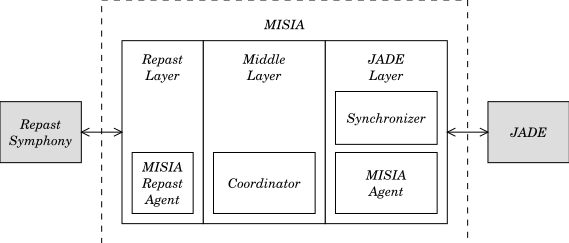
\includegraphics[height=4cm]{figures/MISIA.pdf}
	\end{figure}
\end{frame}

\begin{frame}{JRep}
	Niedersächsische Technische Hochschule (\url{www.nth-online.org})

	\begin{figure}
		\centering
		\includegraphics[height=4cm]{figures/jrep.pdf}
	\end{figure}
\end{frame}

\begin{frame}{PlaSMA}
	TZI, Universität Bremen (\url{www.tzi.de})

	\begin{figure}
		\centering
		\includegraphics[height=4cm]{figures/PlaSMA.pdf}
	\end{figure}
\end{frame}

\begin{frame}{Comparação}
	\begin{itemize}
		\item JRep, MISIA não são projetos ativos
		\item Os três exemplos dependem da plataforma JADE durante a simulação
	\end{itemize}
\end{frame}

%%%%%%%%%%%%%%%%%%%%%%%%%%%%%%%%%%%%%%%%%%%%%%%%%%%%%%
%%%%%%%%%%%%%%%%%%%%%%%%%%%%%%%%%%%%%%%%%%%%%%%%%%%%%%
\subsection{JADE e Repast}

\begin{frame}{JADE}
	\begin{table}[h]
		\label{tab:jadevsrep}
		\tiny
		\begin{center}
			\begin{tabular}{l|cc}
			\hline

			\hline
			\textbf{} & \textbf{JADE} & \textbf{Repast} \\ %& \textbf{Cougaar} \\
			\hline
				Comunicação & FIPA ACL &  Acesso direto  \\ %& Serialized Object \\
							  &			 &  Partilha de recursos \\
			\hline
				Distribuído & Sim & Não \\ 
			\hline
				Simulação & Não & Sim \\ 
			\hline
				Escalabilidade & Limitada & Elevada \\ 
			\hline
				Ontologias & Sim & Não \\
			\hline
				Execução de & Behaviours 	& Escalonamento  	\\ %&  \\
				Agentes		& Multi thread 	& Single thread 	\\ %&  \\
							& Eventos   	& Ticks		 	   	\\ %&  \\
							& Assíncrona 	& Síncrona 		   	\\ %&  \\
			\hline
				Código Livre & Sim & Sim \\ 
			\hline
				Linguagem & Java & Java \\ 
			\hline
			\end{tabular}
		\end{center}
		\caption{Comparação entre JADE e Repast.}
	\end{table}
\end{frame}

%%%%%%%%%%%%%%%%%%%%%%%%%%%%%%%%%%%%%%%%%%%%%%%%%%%%%%
%%%%%%%%%%%%%%%%%%%%%%%%%%%%%%%%%%%%%%%%%%%%%%%%%%%%%%
\subsection{Especificações FIPA no JADE}
\begin{frame}{Especificações FIPA no JADE}
	Três conceitos principais:
		\begin{itemize}
			\item Gestão de Agentes (DF, AMS, AID)
			\item Serviço de Mensagens (MTS, ACL Message)
			\item Protocolos de interação (FIPA Request, FIPA Contract Net)
		\end{itemize}
		
\end{frame}




\section{SAJaS}
%!TEX root = ../thesis.tex

%%%%%%%%%%%%%%%%%%%%%%%%%%%%%%%%%%%%%%%%%%%%%%%%%%%%%%
%%%%%%%%%%%%%%%%%%%%%%%%%%%%%%%%%%%%%%%%%%%%%%%%%%%%%%
\subsection{SAJaS}

\begin{frame}{SAJaS}
	Ações dos agentes são encapsuladas em ``Behaviours''
	
	Duas possibilidades de execução de implementação da comunicação:
	\begin{figure}[!h]
	\centering
		\begin{tikzpicture}
			\pause
			\node (img1) {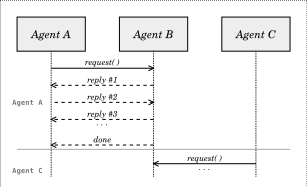
\includegraphics[height=4cm] {../figures/executionProblem.pdf}};
			\node (text1) at (img1.south) [yshift=-0.2cm] {(a) Acesso direto};
			\pause
			\node (img2) {\includegraphics[height=4cm]{../figures/executionProblem2.pdf}};
			\node (text1) at (img2.south) [yshift=-0.2cm] {
				\colorbox{white}{(b) Comunicação assíncrona}};
		\end{tikzpicture}
	\end{figure}

\end{frame}
\begin{frame}{SAJaS}
	Solução para comunicação ``assíncrona'' no SAJaS
	\begin{figure}
		\centering
		\begin{tikzpicture}
			\pause
			\node (img1) {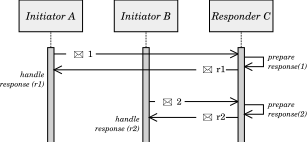
\includegraphics[height=3cm]
				{../figures/tickExample2.pdf}};
			\node (text1) at (img1.south) [yshift=-0.2cm] {JADE};
			\pause
			\node (img2) {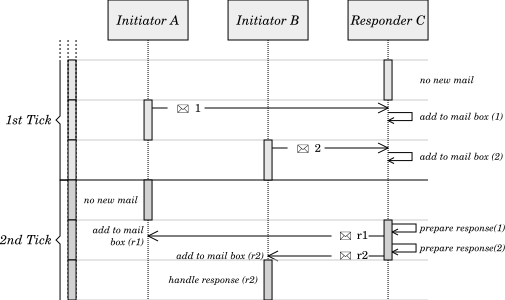
\includegraphics[height=6cm]
				{../figures/tickExample.pdf}};
			\node (text1) at (img2.south) [yshift=-0.2cm] {
				\colorbox{white}{SAJaS}};
		\end{tikzpicture}
	\end{figure}

\end{frame}

\subsection{Arquitetura}
\begin{frame}{Arquitetura}
	\begin{figure}
		\centering
		\begin{tikzpicture}
			\node (img1) {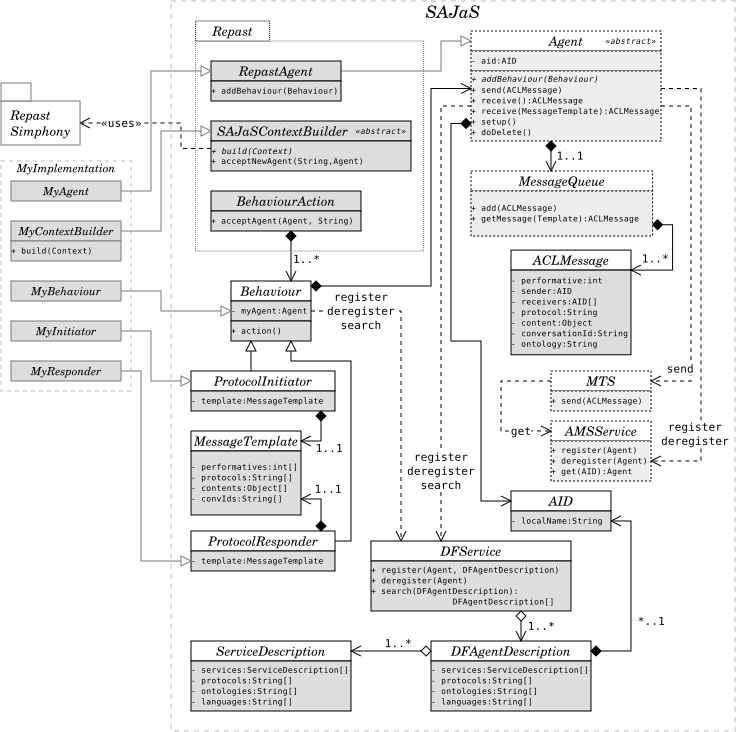
\includegraphics[height=6cm]
				{../figures/sajas_arch.pdf}};
			\node (text1) at (img1.south) [yshift=-0.2cm] {Arquitetura do SAJaS};
			\pause
			\node (img2) {\includegraphics[height=6cm]
				{figures/sajas_arch_simple.pdf}};
			\node (text1) at (img2.south) [yshift=-0.2cm] {
				\colorbox{white}{Arquitetura simplificada do SAJaS}};
		\end{tikzpicture}
	\end{figure}
\end{frame}

\subsection{FIPA}
\begin{frame}{FIPA}
	\begin{figure}
	\centering
	\includegraphics[width=0.7\linewidth]{../figures/sajas_arch_proto_simple.pdf}
	\caption[Behaviours and protocols in SAJaS]
	{Behaviours e Protocolos no SAJaS}
	\label{fig:arch_proto}
\end{figure}
\end{frame}

\section{MASSim2Dev}
%!TEX root = ../thesis.tex

%%%%%%%%%%%%%%%%%%%%%%%%%%%%%%%%%%%%%%%%%%%%%%%%%%%%%%
%%%%%%%%%%%%%%%%%%%%%%%%%%%%%%%%%%%%%%%%%%%%%%%%%%%%%%
\begin{frame}{MASSim2Dev - Ferramenta de Conversão}

	\begin{itemize}
	\item MASSim2Dev (\emph{MAS Simulation to Development code conversion tool})
	\item Estabelece a ponte entre o desenvolvimento e simulação de MAS utilizando o SAJaS
	\end{itemize}
\end{frame}

\subsection{Transformações de código}
\begin{frame}{MASSim2Dev - Ferramenta de Conversão}

	Transformações de código Java

	\begin{itemize}
	\item ATL (``ATLAS Transformation Language'') - transformações de modelos através de AST usando linguagem específica;
	\item Spoon - transformações de código Java baseadas em anotações, usando Java
	\item JDT (``Eclipse Java Development Tools'') - criação de plugins para Eclipse, que permitem edições de alto nível, assim como via AST

	\end{itemize}
\end{frame}

\subsection{Processo de conversão}
\begin{frame}{MASSim2Dev - Ferramenta de Conversão}

	Após a conversão, não restam dependências da plataforma original.
	\begin{figure}[h]
	\centering
	\includegraphics[height=5cm]{../figures/conversion_representation.pdf}
\end{figure}
	
\end{frame}

\section{Validação}
%!TEX root = ../thesis.tex
\chapter{Validation}
\label{chap:validation}

All tests were performed using an Intel i7 CPU (8 logical cores) at 2.20 GHz. 

%!TEX root = ../thesis.tex
\section{Simple Contract Net}

In this scenario, one agent sends a call for proposals (CFP) to multiple agents which then reply with their individual proposals. This simple scenario was created to test the core of SAJaS and the plugin. The goal was not only to create a working simulation model based on SAJaS, but also to demonstrate that the execution of a simulation in SAJaS and the equivalent JADE application generated from it are identical and that performance in SAJaS is higher.

\subsection{Experimental Setup}

The diagram in Figure \ref{fig:CNetExample} illustrates the contract net created for this test. An agent (the buyer) intends to purchase a certain quantity of three kinds of goods: rice, flour and oats. Besides the quantities of each product it needs, the buyer also stipulates a maximum price for the whole deal. The buyer will issue a call for proposals (CFP) containing a request for supplies to all agents that announce themselves as suppliers in the DF.

Supplier agents have a maximum supply capacity and a price for each product. After receiving a CFP, the supplier replies with a PROPOSAL containing a price for each product if the demanded supply is within the seller's capacity. Otherwise, a REFUSE message will be sent to the buyer.
Finally, the buyer agent compares all valid proposals, chooses the cheapest offer for each of the three products and replies with an ACCEPT PROPOSAL to the best offers, and REJECT PROPOSAL to all others.

\begin{figure}[h]
	\centering
	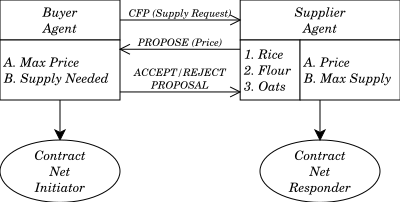
\includegraphics[width=0.60\linewidth]{figures/CNetExample.pdf}
	\caption{Representation of the contract net scenario.}
	\label{fig:CNetExample}
\end{figure}

To ensure the proper comparison of results, a fixed data set with values for prices and demand was used in both frameworks. This experiment focused on two simple metrics to evaluate the result: time and outcome. 

Multiple executions were performed with varying numbers of suppliers (as sugested by Figure \ref{fig:performance}); for each case, the simulation was executed 10 times. The execution time was measured from be begining of the protocol, until all suppliers were notified.

In JADE, the simulation was tested in two different setups: first, with all agents running in a single container; second, with the supplier agents in one container and the buyer in a separate one (but in the same host). In this configuration, all communication between agents happens across containers. The second validation metric was the actual result of the protocol, i.e who were the supplier agents chosen by the buyer and their price proposals.

\subsection{Results}

For each number of agents, the experiment was run 10 times. The average performance of of the experiment for each number of agents is represented in Figure \ref{fig:performance}. The performance of the simulation based on SAJaS was significantly better, excelling when the number of agents is high. JADE was able to perform better when using two distinct containers. JADE's performance drops very significantly when there is a high communication-to-computation ratio in the application. Also, JADE is capable of performing some optimizations when two interacting agents are located within the same containers\cite{mengistu2008scalability}.

Regarding the outcome of the protocol, the same values were obtained in both implementations for each number of agents, confirming that the execution is identical in both implementations.

\begin{figure}[h]
	\centering
	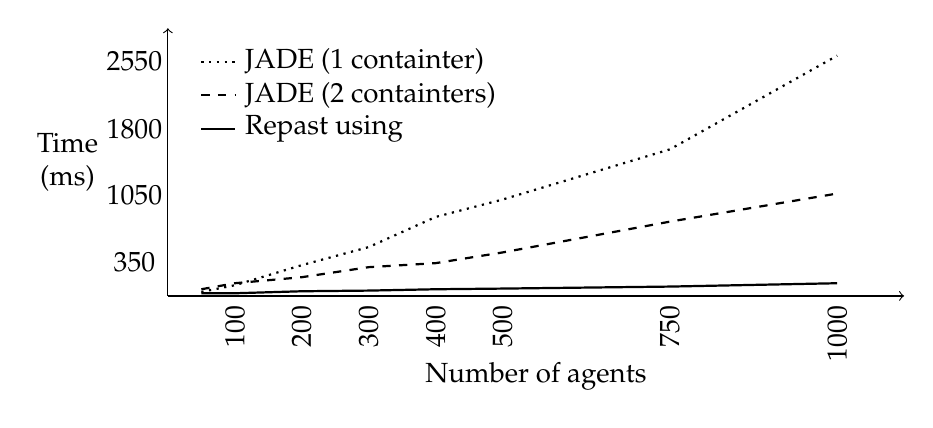
\begin{tikzpicture}[scale=0.85]

		% horizontal axis
		\draw[->] (0,0) -- (11,0);
		\draw (5.5,-1.2) node[align=center] {Number of agents}; %label

		
		% labels
		\draw	%(0.5,0) node[rotate=90, anchor=east] {50}
				(1.0,0) node[rotate=90, anchor=east] {100}
				(2.0,0) node[rotate=90, anchor=east] {200}
				(3.0,0) node[rotate=90, anchor=east] {300}
				(4.0,0) node[rotate=90, anchor=east] {400}
				(5.0,0) node[rotate=90, anchor=east] {500}
				(7.5,0) node[rotate=90, anchor=east] {750}
				(10.,0) node[rotate=90, anchor=east] {1000};

		\draw	(-0.5,0.5) node[anchor=center] {350}
				(-0.5,1.5) node[anchor=center] {1050}
				(-0.5,2.5) node[anchor=center] {1800}
				(-0.5,3.5) node[anchor=center] {2550};
		% vertical axis
		\draw[->] (0,0) -- (0,4);
		\draw (-1.5,2) node[align=center] {Time\\(ms)}; %label
		%\draw (-1.5,1.6) node[align=center] {(ms)}; %label

		%% Data %%
		% JADE 2 containers
		\draw[thick,dashed] (0.5,3.0) --
			(1,3.0) node[anchor=west, pos=1.0] {JADE (2 containters)}; %subtitle
		\draw[thick,dashed] (0.5, 0.10) --
					(1.0, 0.19) --
					(2.0, 0.28) --
					(3.0, 0.43) --
					(4.0, 0.49) --
					(5.0, 0.65) --
					(7.5, 1.11) --
					(10., 1.53);
		% JADE 1 containers
		\draw[thick,dotted] (0.5,3.5) --
			(1,3.5) node[anchor=west, pos=1.0] {JADE (1 containter)}; %subtitle
		\draw[thick,dotted] (0.5, 0.06) --
					(1.0, 0.16) --
					(2.0, 0.46) --
					(3.0, 0.73) --
					(4.0, 1.18) --
					(5.0, 1.44) --
					(7.5, 2.19) --
					(10., 3.59);
		% Repast
		\draw[thick] (0.5,2.5) --
			(1,2.5) node[anchor=west, pos=1.0] {Repast using \apiname{}}; %subtitle
		\draw[thick] (0.5, 0.04) --
					(1.0, 0.04) --
					(2.0, 0.07) --
					(3.0, 0.08) --
					(4.0, 0.10) --
					(5.0, 0.11) --
					(7.5, 0.14) --
					(10., 0.19);


	\end{tikzpicture}
	\caption[Execution performance in a simple contract net]
	{Average execution time of each framework in the different experiments.}
	\label{fig:performance}
\end{figure}

%!TEX root = ../thesis.tex
\section{Multiple Contract Net using Trust}

This scenario is similar to the previous one, but attempts to perform a better coverage of the features present in SAJaS, namely the use of the AchieveRE Protocol and the Responder Dispatcher which allows for multiple contract nets to be handled without deadlocks occuring. However. rather than comparing the exact value obtained from the simulation as in the previous scenario, the goal is to compare the overall behaviour of all agents.

\subsection{Experimental Setup}
This simulation is composed by multiple buyers and multiple sellers running simultaneously. After the sellers register themselves in the DF, each buyer will perform a search for sellers of the particular good it needs to purchase. Then, the buyer sends this list of agents to the CTAgent (CT standing for computational trust). The CTAgent will calculate a trust value for each seller based on its past contracts with buyers and return the top 5 sellers.

With this information, the buyer sends a CFP only to the 5 top agents and accept the best proposal from them. Some sellers will occasionally violate the contract after acceptance. The buyer will then inform the CTAgent if the contract was fulfilled or violated. The compilation of this composes the trust of the seller.

Some buyers are programmed to ignore trust and rely solely on the proposal. The idea is that informed buyers eventually avoid contacting sellers programmed to violate contracts more often. The goal of this experiment is to model this scenario in SAJaS, convert it to JADE and verify that the obtained results are very similar.

After one contract is concluded, Buyers start a new one, performing a new DF search for the next product they want to buy, request information from the CTAgent and issuing a new CFP.

\subsection{Results}

The experiment was executed 5 times in JADE and 5 times in SAJaS. The scenario is composed of 20 buyers using computational trust, 20 not using trust and 80 sellers. A total of 2000 contracts were recorded to create the following charts in Figures \ref{fig:enterprise_JADE} and \ref{fig:enterprise_SAJaS}. As shown, buyers who made use of computational trust had more successful contracts. The fluctuations early in the simulation are due to the initial lack of trust information.

As expected and as shown in the charts, the same outcome was observed both in JADE and SAJaS. With this experiment, it was possible to test the Request protocol - when requesting computational trust, the Contract Net - when purchasing goods, the Responder Dispatcher - to handle CFPs from multiple buyers concurrently, the messaging system and the DF service.

In terms of performance, the outcome of this experiment, as ilustrated by the chart in Figure \ref{fig:enterprise_times}, may not seem as impressive when compared with the first experience. However, the algorithm employed to calculate trust is very time consuming. In a setup without the use of trust by any of the buyers, the performance difference between JADE and SAJaS is comparable to the first scenario.

\begin{figure}[ht]
	\centering
	\begin{subfigure}[b]{\textwidth}
		\centering
		\begin{tikzpicture}[scale=0.85]

			% horizontal axis
			\draw[->] (0,0) -- (11,0);
			\draw (5.5,-1.2) node[align=center] {Number of Contracts}; %label

			% labels
			\draw	(0  ,0) node[anchor=north] {0}
					(2.5,0) node[anchor=north] {500}
					(5  ,0) node[anchor=north] {1000}
					(7.5,0) node[anchor=north] {1500}
					(10 ,0) node[anchor=north] {2000};
			
			
			% vertical axis
			\draw[->] (0,0) -- (0,5);
			\draw (-1.1,2.5) node[rotate=90, anchor=south, align=center]
				{\% of Fullfielment}; %label
			\draw	(0, 1) node[anchor=east] {0.25}
					(0, 2) node[anchor=east] {0.50}
					(0, 3) node[anchor=east] {0.75}
					(0, 4) node[anchor=east] {1.00};
			
			

			%% Data %%

			%subtitles
			\draw[thick] (0.5,3.5) --
				(1,3.5) node[anchor=west, pos=1.0] {Using trust and proposal};
			\draw[thick, dotted]
				(0.5,4.5) --
				(1,4.5) node[anchor=west, pos=1.0] {Using only the proposal}; 

			%lines
			\input{chapters/charts/enterprise_values_jade}


		\end{tikzpicture}
		\caption{In SAJaS}
		\label{fig:enterprise_JADE}
	\end{subfigure}
	\bigskip\\
	\begin{subfigure}[b]{\textwidth}
		\centering
		\begin{tikzpicture}[scale=0.85]

			% horizontal axis
			\draw[->] (0,0) -- (11,0);
			\draw (5.5,-1.2) node[align=center] {Number of Contracts}; %label

			% labels
			\draw	(0  ,0) node[anchor=north] {0}
					(2.5,0) node[anchor=north] {500}
					(5  ,0) node[anchor=north] {1000}
					(7.5,0) node[anchor=north] {1500}
					(10 ,0) node[anchor=north] {2000};
			
			
			% vertical axis
			\draw[->] (0,0) -- (0,5);
			\draw (-1.1,2.5) node[rotate=90, anchor=south, align=center]
				{\% of Fullfielment}; %label
			\draw	(0, 1) node[anchor=east] {0.25}
					(0, 2) node[anchor=east] {0.50}
					(0, 3) node[anchor=east] {0.75}
					(0, 4) node[anchor=east] {1.00};

			%% Data %%

			%subtitles
			\draw[thick] (0.5,3.5) --
				(1,3.5) node[anchor=west, pos=1.0] {Using trust and proposal};
			\draw[thick, dotted] 
				(0.5,4.5) --
				(1,4.5) node[anchor=west, pos=1.0] {Using only the proposal}; 
			
			%lines
			\input{chapters/charts/enterprise_values_sajas}


		\end{tikzpicture}
		\caption{In JADE}
		\label{fig:enterprise_SAJaS}
	\end{subfigure}
	\caption[Multiple Contract Net scenario results in JADE]
	{Average result of 5 executions of the Multiple Contract Net scenario during 2000 contracts}
\end{figure}

\begin{figure}
	\centering
	\begin{tikzpicture}[scale=0.85]

		% horizontal axis
		\draw[->] (0,0) -- (11,0);
		\draw (5.5,-1.2) node[align=center] {Time/s}; %label

		% labels
		\draw	(1.4,0) node[anchor=north] {2}
				(2.8,0) node[anchor=north] {4}
				(4.2,0) node[anchor=north] {6}
				(5.6,0) node[anchor=north] {8}
				(7.1,0) node[anchor=north] {10}
				(8.5,0) node[anchor=north] {12}
				(9.9,0) node[anchor=north] {14};
		
		
		% vertical axis
		\draw[->] (0,0) -- (0,5);
		\draw (-1.1,2.5) node[rotate=90, anchor=south, align=center]
			{Number of Contracts}; %label
		\draw	(0, 0) node[anchor=north] {0}
				(0, 1) node[anchor=east] {500}
				(0, 2) node[anchor=east] {1000}
				(0, 3) node[anchor=east] {1500}
				(0, 4) node[anchor=east] {2000};
		
		

		%% Data 
		%subtitle
		\draw[thick] (0.5,3.5) --
			(1,3.5) node[anchor=west, pos=1.0] {SAJaS};
		%line
		\input{chapters/charts/enterprise_times}

		\draw[thick, dotted]%subtitle
			(0.5,4.5) --
			(1,4.5) node[anchor=west, pos=1.0] {JADE}; 


	\end{tikzpicture}
	\caption[Multiple Contract Net scenario results in Repast]
	{Number of contracts executed in JADE and SAJaS. Final number of contracts is 2000 for both frameworks.}
	\label{fig:enterprise_times}
\end{figure}

\section{Risk Multiplayer Game}

\section{Summary}


\section{Referências}
\bibliography{myrefs}


\end{document}

